\documentclass[prb,preprint]{revtex4-1} 
% The line above defines the type of LaTeX document.
% Note that AJP uses the same style as Phys. Rev. B (prb).

\usepackage{amsmath}  % needed for \tfrac, \bmatrix, etc.
\usepackage{amsfonts} % needed for bold Greek, Fraktur, and blackboard bold
\usepackage{graphicx} % needed for figures
\usepackage{tabularx}

\begin{document}

\title{Optical Pumping of Rubidium OP1-A}
% In a long title you can use \\ to force a line break at a certain location.

\author{Yumeng Melody Cao}
\email{mcao@smith.edu} 
\affiliation{Department of Physics, Smith College, Northampton, MA 01063}
\author{He Claudia Yun}
\email{hyun@smith.edu}
\affiliation{Department of Physics, Smith College, Northampton, MA 01063}

% See the REVTeX documentation for more examples of author and affiliation lists.

\date{\today}

%____________abstract____________________________________________

\begin{abstract}

\end{abstract}

\maketitle 

%____________Introduction____________________________________________
\section{Introduction}

In quantum mechanics, hydrogen-like atoms, i.e. atoms with only one valence electron, are modeled such that the outmost electron can only exist in some discrete energy levels. These orbits are described by quantum numbers $n$ and $l$, where $n=1, 2, ...$ and $l=s, p, d, f, ...$, denoting the energy and orbital angular momentum of the electron. However, this model does not consider the spin of the electron. When the spin is taken into account, each energy level will split into two due to the coupling effect between the spin and the orbital angular momentum of the electron. This is known as the fine structure. The summation $J=L+S$ is the total angular momentum, where $S$ is the electron spin and $L$ is the orbital angular momentum. If the spin of the nucleus $I$ is also considered, each fine-structure level will again split. And the atom will have a total angular momentum $F=I+J$. This is also known as the hyperfine structure. Finally, when a relatively weak external magnetic field is applied, each $F$ level splits into different $M$ levels with spacing proportional to the strength of the field. This splitting is known as the Zeeman effect. The Zeeman splitting is given by

\begin{equation}
E_{z}=g_{F} \mu_{0} BM
\label{zeeman}
\end{equation}

Where $E_{z}$ is the Zeeman energy, the energy difference between two different $M$ levels, B is the external magnetic field strength, and $\mu_{0}$ is the Bohr magneton. 

\begin{equation}
\mu_{0}=\frac{e\hbar}{2m_{e}}=9.27\times10^{-24} J/T
\label{mu0}
\end{equation}

And $g_{F}$ is the coupling constant, known as the Lande g-factor. 

\begin{equation}
g_{F}=g_{J} \frac{F(F+1)+J(J+1)-I(I+1)}{2F(F+1)}
\label{gf}
\end{equation}
and
\begin{equation}
g_{J}=1+\frac{J(J+1)+S(S+1)-L(L+1)}{2J(J+1)}
\label{gj}
\end{equation}

\begin{figure}[h]
\centering
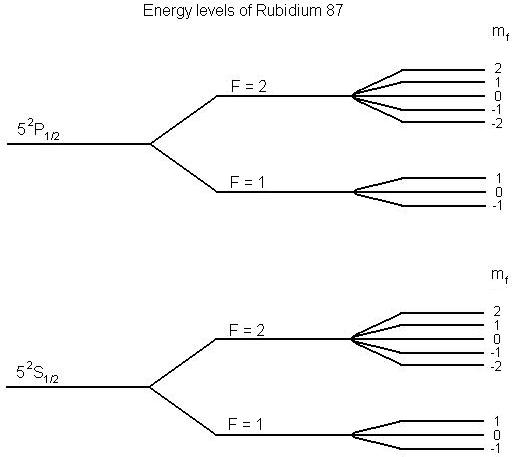
\includegraphics[width=10cm]{energylevels.jpg}
\caption{Zeeman splitting of Rubidium 85 atom \cite{energy}}
\label{energylevels}
\end{figure}

Fig. \ref{energylevels} shows the Zeeman splitting of a Rubidium 87 atom. \\

When a photon with the right energy to excite the electron from level $1s$ to $2p$ enters the atom, the hyperfine levels are so close together that there is an equal possibility of the electron landing in any $F$ level with any $M$. However, there are certain rules the electron has to follow, one of which is that the electron's $M$ value cannot be altered by more than 1. This is to say, $\Delta M=-1, 0, 1$. $\Delta M$ is decided by the nature of the photon. When the applied magnetic field is parallel to the direction of propagation of the photon, a right-circularly-polarized photon will always give $\Delta M=1$ and a left-circularly-polarized photon will give $\Delta M=-1$. The rule also applied to emission. For example, when the electron falls from $2p$ back to $1s$, $\Delta M$ is equally likely to be 1, 0, and -1, so the average $\Delta M=0$. \\

In out experiment, a right-circularly-polarized laser beam with the right frequency to excite electrons from ground state to first excited state passes through some Rubidium vapor and is then detected by a photodiode. Because of the polarization of the photons, transitions induced all have $\Delta M=1$. The average emissions have average $\Delta M=0$, so very quickly all the electrons will be "pumped" up to the highest $M$ level. When that happens, the Rubidium vapor is unable to absorb any more photon, which means that it has become transparent to the laser beam. Then an RF (Radio Frequency) signal is introduced into the system. When the RF signal has the exact energy between the Zeeman splitting, it "depumps" the electrons from the highest $M$ level down, and the Rubidium vapor can absorb photons again, which will cause a sudden decrease in the intensity of the laser beam detected by the photodiode. \\

From Eq. \eqref{zeeman} it can be seen that $E_{z}$ is linearly proportional to $B$. By changing the RF signal, which will match $E_{z}$, and the magnetic field $B$, we could find out the coupling constant $g_{F}$ for Rubidium.\\

%____________Experiment____________________________________________
\section{Experiment}

To implement the optical pumping process, we used the apparatus shown in Fig. 
\ref{exp}, manufactured by TeachSpin Inc. \\

\begin{figure}[h]
\centering
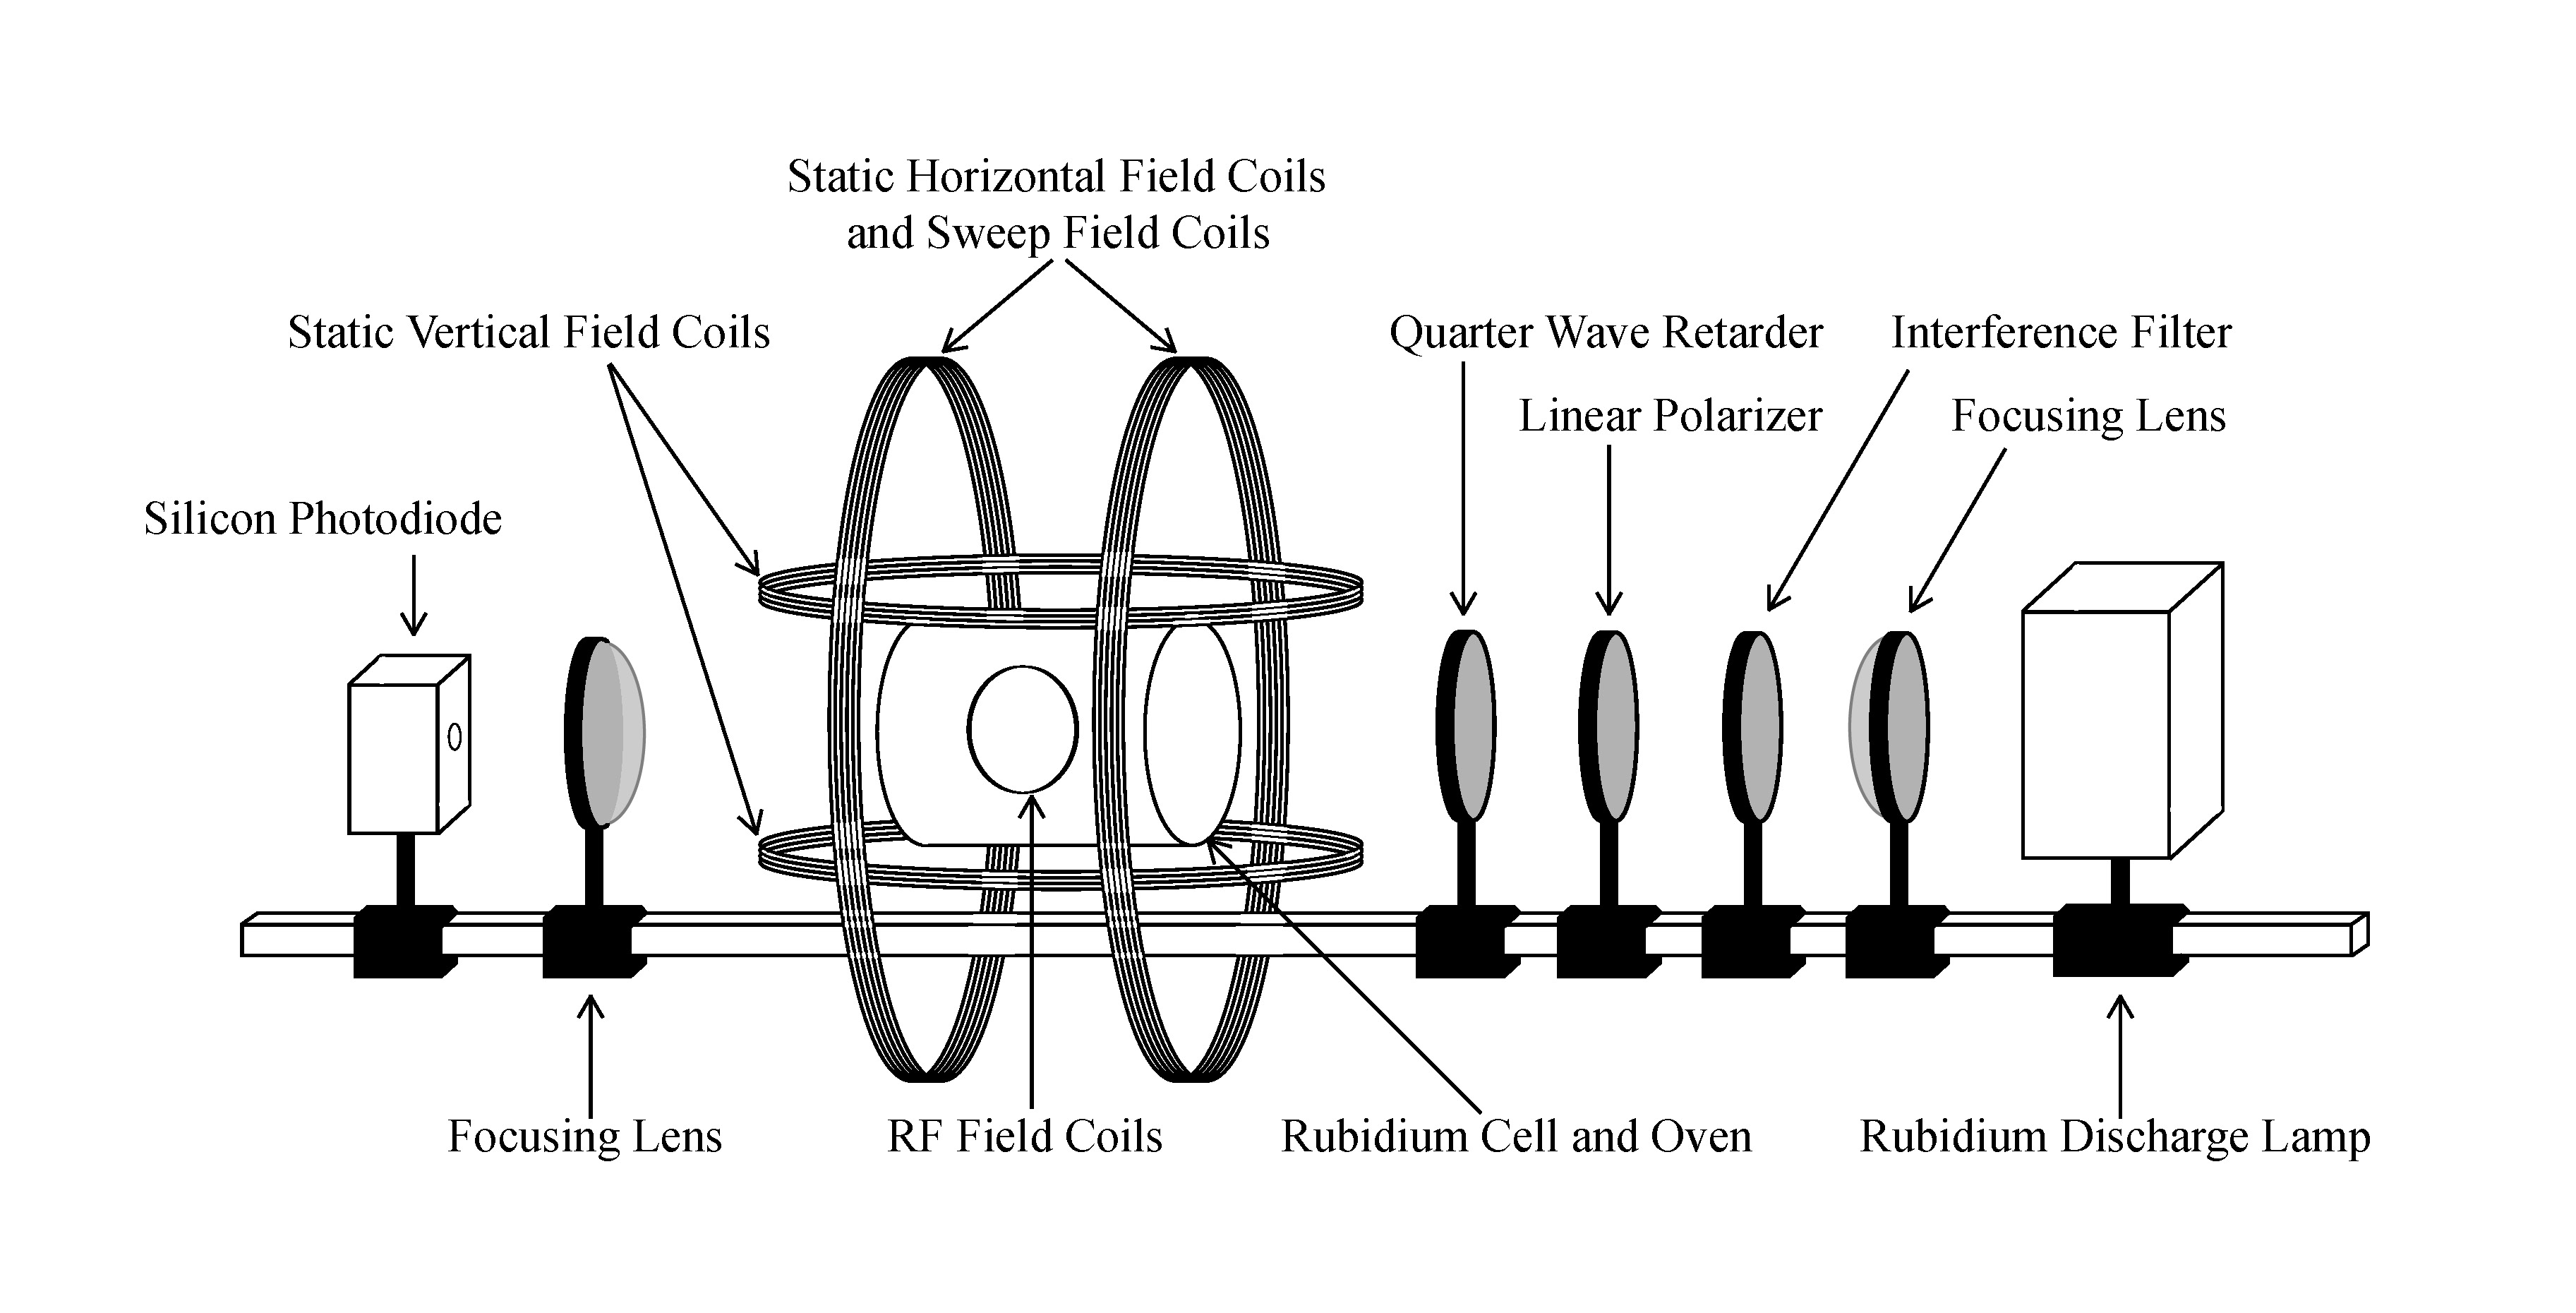
\includegraphics[width=16cm]{exp.jpg}
\caption{Optical pumping of Rubidium apparatus}
\label{exp}
\end{figure}

On the right side of the optical rail, the interference filter limits the bandwidth of light with a pass band of 790 nm to 830 nm, and the linear polarizer and quarter wave retarder convert the light from random polarization to circular polarization. The circular polarized light mandates only $\Delta M=+1$ electric dipole transitions in the atom.The Helmholtz coils provide the magnetic fields, are driven by dial controlled variable voltage dividers, and are monitored by two Agilent 34410 digital multimeters and a Tektronix 2024B oscilloscope. The left side of the optical rail measures the intensity of light passing through the sample which in effect allows us to see when the sample is driven out of the optically pumped state. This signal is also monitored by the oscilloscope. The RF field coils are driven by an HP33120A function generator and drive the sample out of the optically pumped state when the sweep field is at resonance.


%____________Results____________________________________________
\section{Results}

A series of plots of photodiode voltage versus horizontal sweep voltage are obtained at different RF frequency. The horizontal sweep voltage is translated into sweep magnetic field strength by
\begin{equation}
B_{sweep}=8.991\times10^{-3} I N R_{coil}^{-1}
\label{vtob}
\end{equation}

where

\begin{equation}
I=\frac{V_{sweep}/gain}{R}
\label{vtoi}
\end{equation}

R is the sense resistor, which is $1 \Omega$. $N=11$ is the number of wires wrapped on each side and$R_{coil}=0.1639m$ is the average radius of the loop. Gain is 10 in this experiment. \\

\begin{figure}[h]
\centering
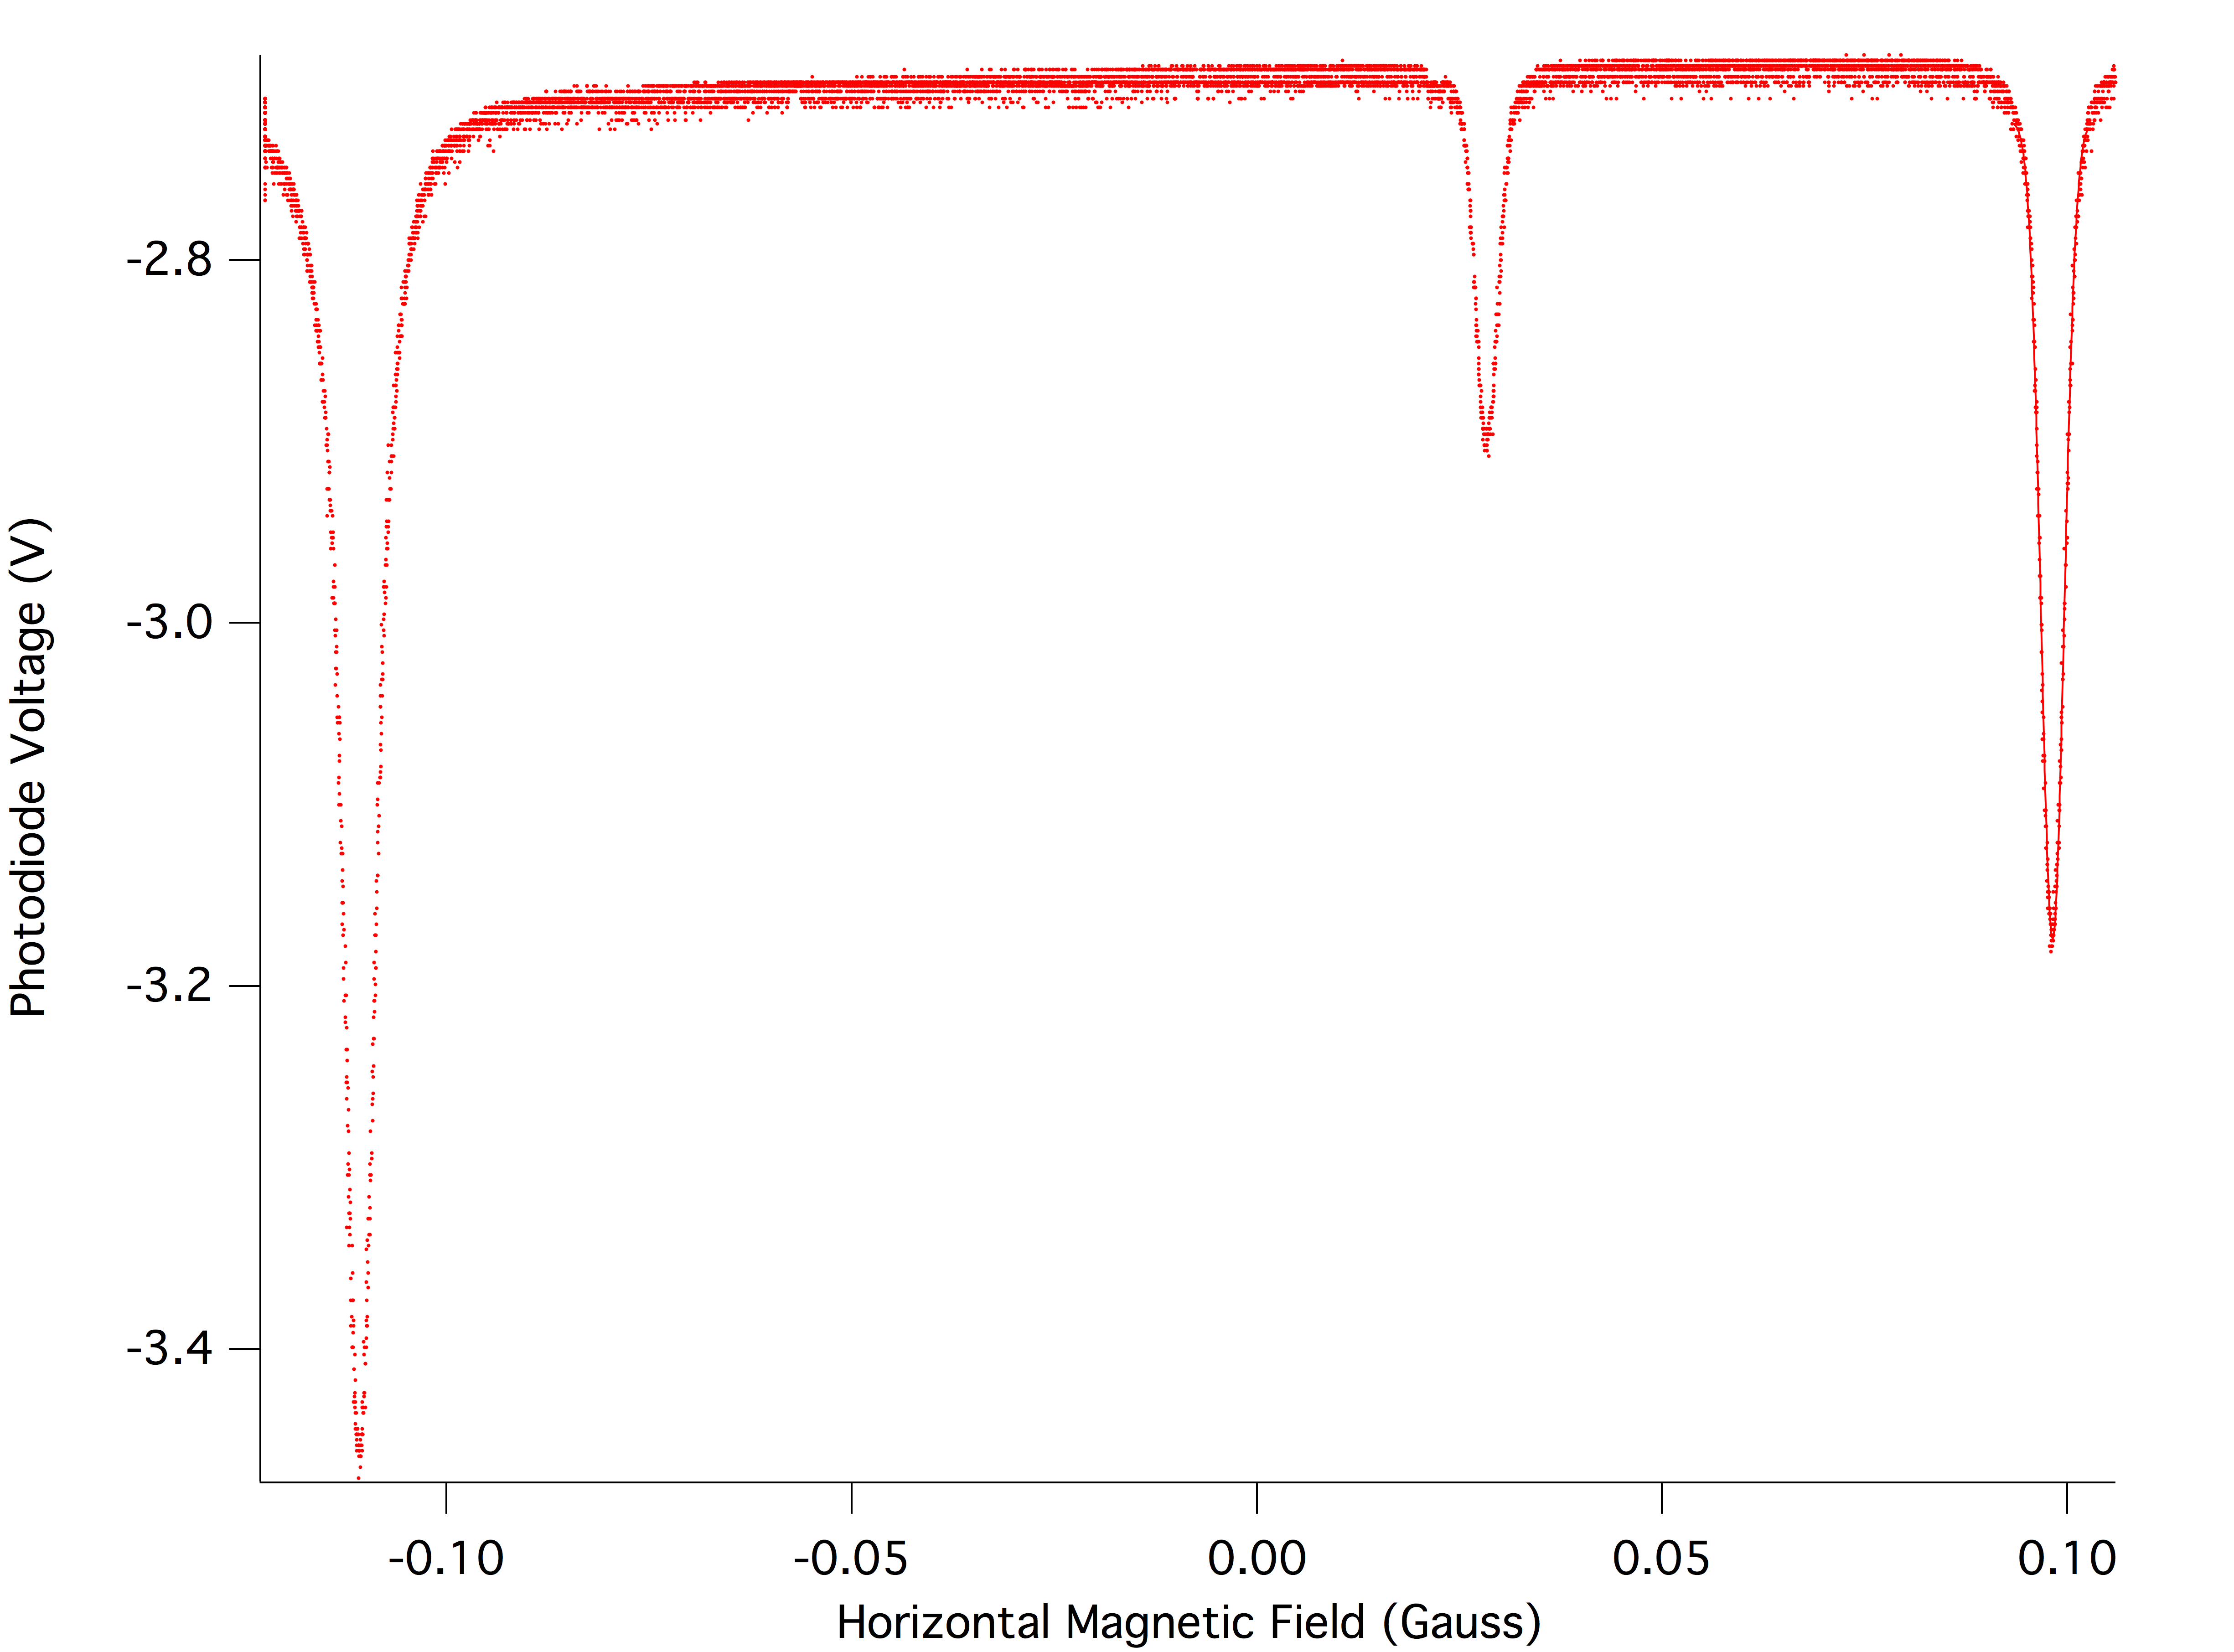
\includegraphics[width=16cm]{100kHz.png}
\caption{Photodiode voltage versus magnetic field strength at 100 kHz. The left trough is the zero field resonance, the middle trough is RF absorption for $^8$$^7$Rb and the right trough is for $^8$$^5$Rb.}
\label{100kHz}
\end{figure}


\begin{figure}[h]
\centering
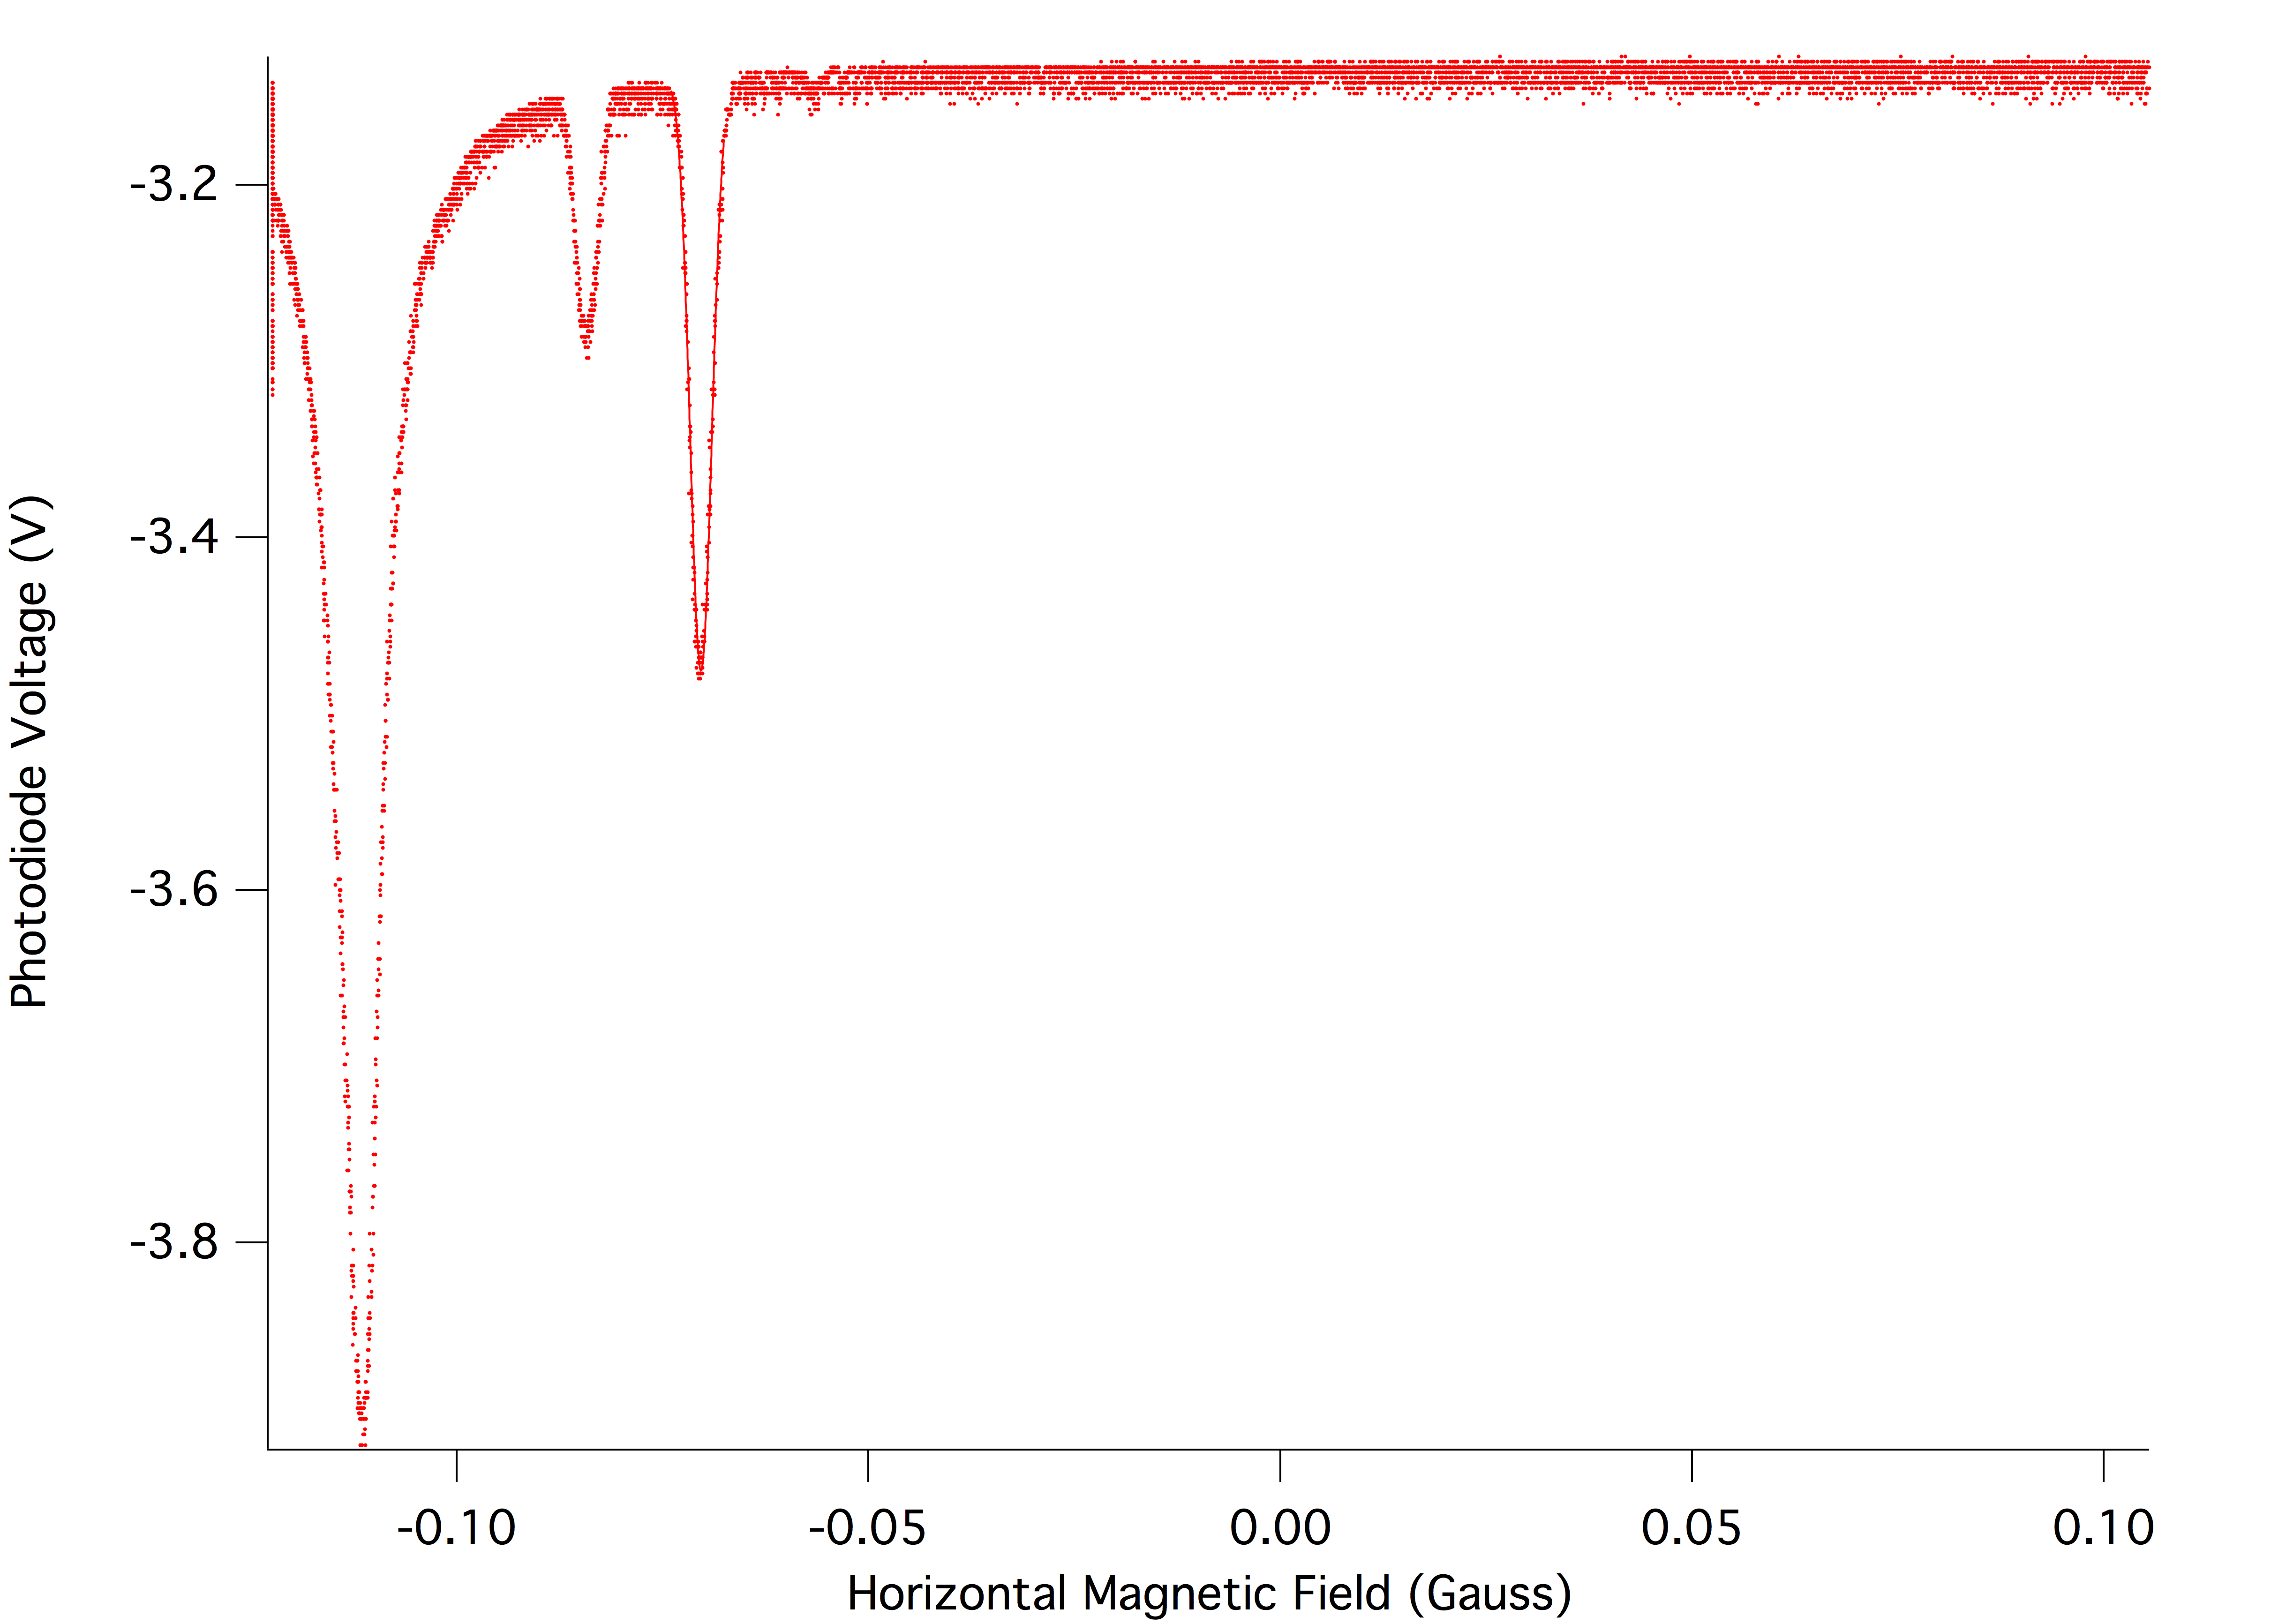
\includegraphics[width=16cm]{20kHz.png}
\caption{Photodiode voltage versus magnetic field strength at 20 kHz. The left trough is the zero field resonance, the middle trough is RF absorption for $^8$$^7$Rb and the right trough is for $^8$$^5$Rb.}
\label{20kHz}
\end{figure}

Fig. \ref{100kHz} and Fig. \ref{20kHz} are two of the plots after the horizontal sweep voltage is converted to magnetic field strength. The first dip is where zero field transition happens, the first dip is where the  $^8$$^7$Rb transition happens and the second dip is the $^8$$^5$Rb transition. The difference between the zero field transition and the Rb transition is calculated to find the true magnetic field that is resonant with a given RF frequency. The resonant magnetic field is found for both $^8$$^7$Rb and $^8$$^5$Rb at RF frequency varying from 10kHz to 100kHz with a step size of 10kHz, and is also plotted versus the RF frequencies. Table. \ref{data} shows the positions of the dips and the resonant fields with uncertainties. Fig. \ref{both} shows the plot, from which it can be seen that resonant magnetic field and RF frequencies have a linear relationship. The different depth of the dips are caused by different amount of $^8$$^7$Rb and $^8$$^5$Rb in nature. There is more $^8$$^5$Rb than $^8$$^7$Rb, so the second dip is deeper. However, the photodiode voltage is not used for any calculation in this experiment. So we will not analyze it in detail.

\begin{table}[h]
\centering
\caption{Optical pumping resonance field data}
\begin{ruledtabular}
\begin{tabular}{ l c c c}
RF & Zero Field Dip & Rb87 Dip & Rb85 Dip\\
(kHz) & (Gauss) & (Gauss) & (Gauss)\\
\hline
100	& -0.33216$\pm$2.40E-05 & 0.08509$\pm$1.80E-05 & 0.29449$\pm$1.44E-05\\
90&-0.33221$\pm$2.37E-05&0.042623$\pm$2.09E-05&0.22929$\pm$1.61E-05\\
80&-0.33336$\pm$2.79E-05&0.00052957$\pm$1.90E-05&0.16733$\pm$1.23E-05\\
70&-0.33167$\pm$3.33E-05&-0.040531$\pm$2.51E-05&0.10456$\pm$1.51E-05\\
60&-0.33178$\pm$2.96E-05&-0.082066$\pm$2.36E-05&0.041789$\pm$1.62E-05\\
50&-0.33256$\pm$3.65E-05&-0.12408$\pm$2.52E-05&-0.019752$\pm$1.86E-05\\
40&-0.33227$\pm$3.11E-05&-0.16902$\pm$3.25E-05&-0.082741$\pm$2.29E-05\\
30&-0.33257$\pm$3.25E-05&-0.20774$\pm$3.69E-05&-0.1458$\pm$2.44E-05	\\
20&-0.33519$\pm$3.26E-05&-0.2527$\pm$3.73E-05&-0.2111$\pm$2.93E-05\\
10	&-0.335555$\pm$3.79E-05&-0.29493$\pm$7.74E-05&-0.27365$\pm$3.03E-05\\

\end{tabular}
\end{ruledtabular}
\label{data}
\end{table}

\begin{table}[h]
\centering
\caption{Optical pumping resonance field data (continued)}
\begin{ruledtabular}
\begin{tabular}{ l c c}
RF & RB87 Resonant Field & RB85 Resonant Field\\
(kHz) & (Gauss) & (Gauss)\\
\hline
100 & 0.41725$\pm$4.20E-05 & 0.62665$\pm$3.84E-05\\
90 & 0.374833$\pm$4.46E-05 & 0.5615$\pm$3.98E-05\\
80 & 0.33388957$\pm$4.69E-05 & 0.50069$\pm$4.02E-05\\
70 & 0.291139$\pm$5.84E-05 & 0.43623$\pm$4.84E-05\\
60 & 0.249714$\pm$5.32E-05 & 0.373569$\pm$4.58E-05\\
50 & 0.20848$\pm$6.17E-05 & 0.312808$\pm$5.51E-05\\
40 & 0.16325$\pm$6.36E-05 & 0.249529$\pm$5.40E-05\\
30 & 0.12483$\pm$6.94E-05 & 0.18677$\pm$5.69E-05\\
20 &	0.08249$\pm$6.99E-05 & 0.12409$\pm$6.19E-05\\
10 &	0.040625$\pm$1.15E-04 & 0.061905$\pm$6.82E-05\\

\end{tabular}
\end{ruledtabular}
\label{data2}
\end{table}



\begin{figure}[h]
\centering
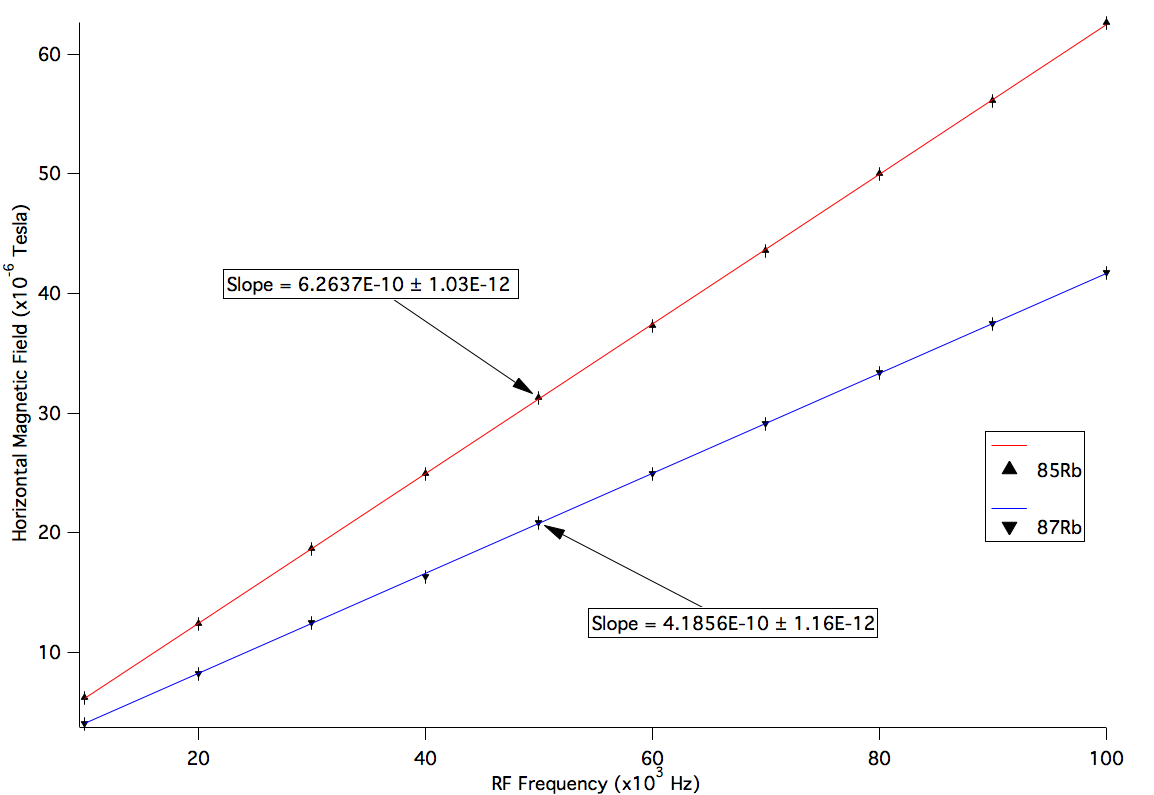
\includegraphics[width=16cm]{both.png}
\caption{Horizontal magnetic field strength in resonance vs. RF frequency}
\label{both}
\end{figure}

The $^8$$^7$Rb and $^8$$^5$Rb scatter plots are separately fitted by lines. The slope of the $^8$$^7$Rb is $4.1856\times 10^{-10} \pm 1.16 \times 10^{-12}$ and the slope of the $^8$$^5$Rb is $6.2637 \times 10^{-10} \pm 1.03 \times 10^{-12}$. Resonance only occurs when the RF signal has the right energy to depump the electrons. The "right" energy here is the Zeeman energy, which is the difference in energy between two neighbor $M$ levels. \\

The energy of the RF signal is given by
\begin{equation}
E_{RF}=h\nu
\label{rfenergy}
\end{equation}

Let $E_{RF}=E_{z}$ in Eq. \ref{zeeman} and move the terms around, we get
\begin{equation}
B=\frac{h}{g_{F}\mu_{0}}\nu
\label{bandf}
\end{equation}

where B is the the resonant magnetic field and $\nu$ is the RF frequency. And it is easy to see that they have a linear relationship. $g_{F}$ can be calculate from the slope of the fit line:

\begin{equation}
g_{F}=\frac{\mu_{0}}{h} \times \frac{1}{Slope}
\label{gf}
\end{equation}

$g_{F}$ is found to be $0.1708\pm0.0004$ for $^8$$^7$Rb and $0.1141\pm0.0002$ for $^8$$^5$Rb where the expected values are 1/2 and 1/3.



%____________Discussion____________________________________________
\section{Discussion}
The experimental $g_{F}$ values are inconsistent with the expected values, both of which are about 3 times bigger.\\
The first possibility that could cause this discrepancy is that there is an unknown magnetic field $B_{unknown}$ that is either not counted or over counted in Eq. \ref{zeeman}. 

\begin{equation}
B_{true}^{2}=B^{2}+B_{unknown}^{2}
\label{bnew}
\end{equation}

where B is the magnetic field value we are currently using. To test out this hypothesis, the theoretical value of $g_{F}$ of $^8$$^5$Rb is employed to calculate $B_{true}$ and thus find out $B_{unknown}$. Then this additional magnetic field is added to the measured resonant magnetic field of the other isotope and thus find out its $g_{F}$ factor. \\

\begin{table}[h]
\centering
\caption{$B_{unknown}$}
\begin{ruledtabular}
\begin{tabular}{ l c c c}
RF & RB85 Resonant Field & RB85 Resonant Field & Unknown Magnetic Field squared\\
 & (Measured) & (Calculated) & \\
(kHz) & (Gauss) & (Gauss) & (Gauss$^{2}$)\\
\hline
100 & 0.41725 & 0.214434 & -0.346708\\
90 & 0.374833 & 0.19299 & -0.278037\\
80 & 0.33388957 & 0.171547 & -0.221262\\
70 & 0.291139 & 0.150104 & -0.167766\\
60 & 0.249714 & 0.12866 & -0.123\\
50 & 0.20848 & 0.107217 & -0.0863534\\
40 & 0.16325 & 0.0857735 & -0.0549076\\
30 & 0.12483 & 0.0643301 & -0.0307447\\
20 &	0.08249 & 0.0428867 & -0.0135591\\
10 &	0.040625 & 0.0214434 & -0.00337241\\

\end{tabular}
\end{ruledtabular}
\label{calibration}
\end{table}

It is noticeable that the square of the unknown magnetic field is negative. This actually makes sense, because from Fig. \ref{caliplot} it can be seen that the calculated values are always smaller than the measured ones.

\begin{figure}[h]
\centering
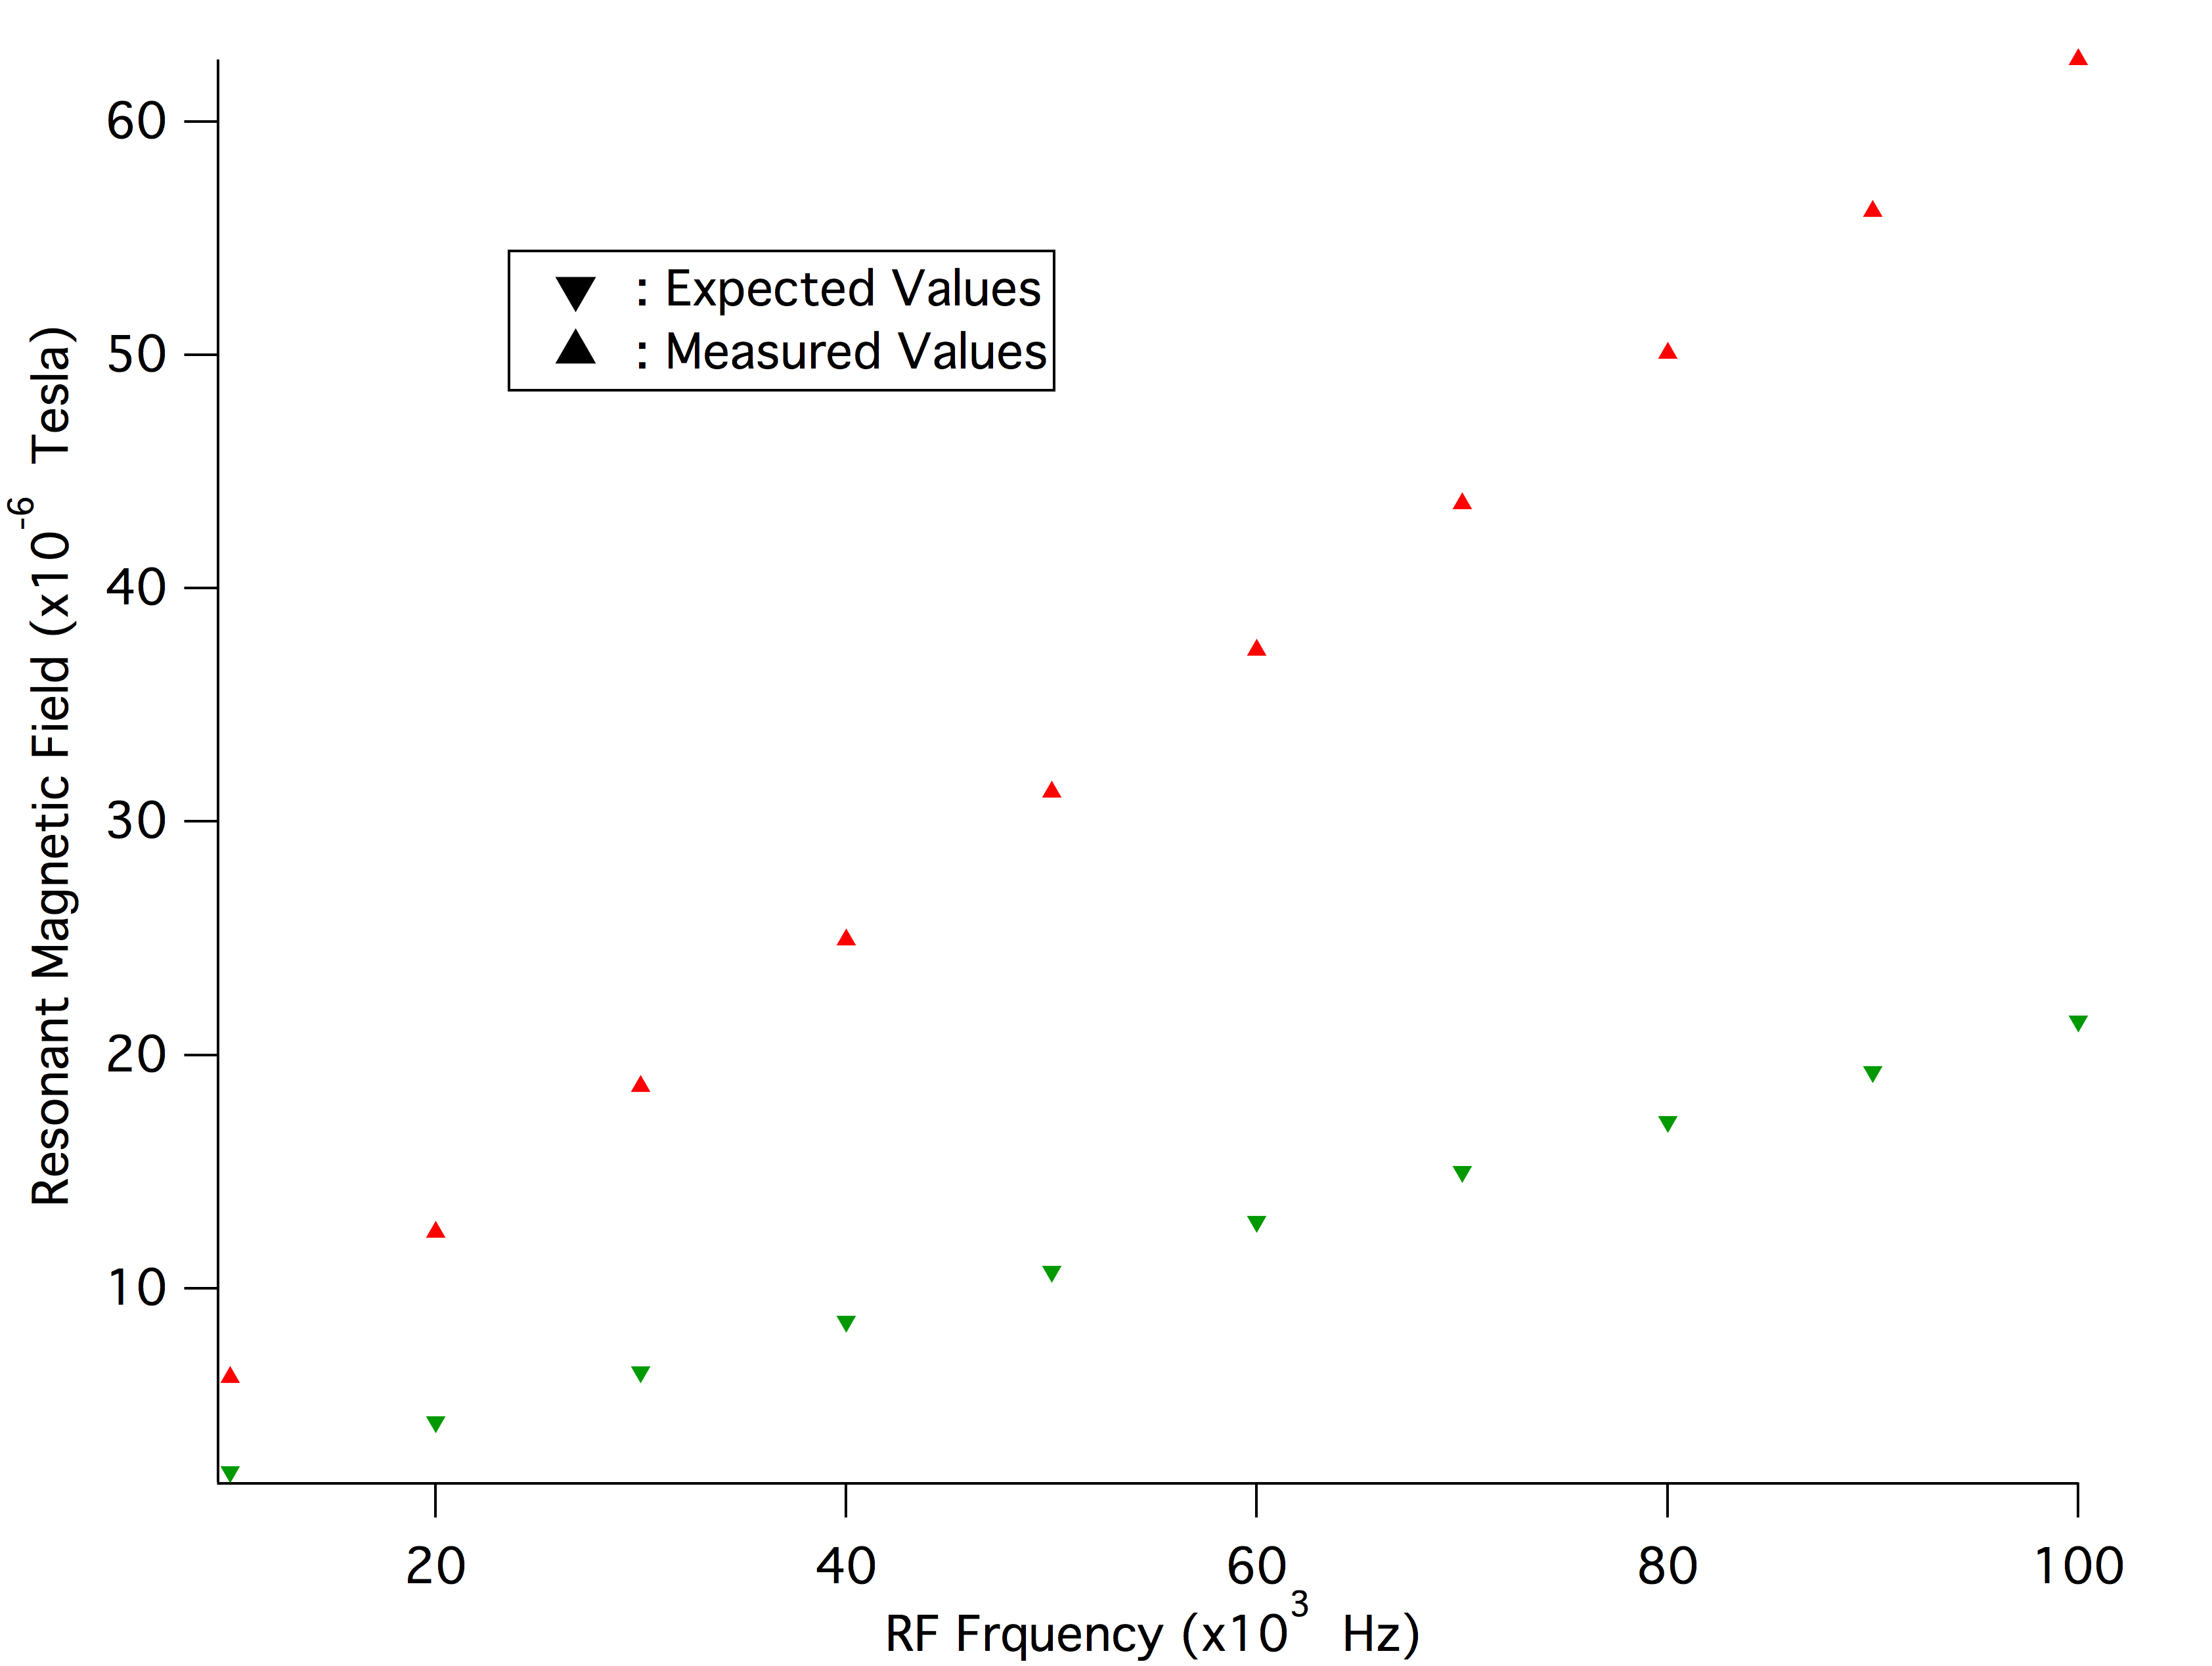
\includegraphics[width=16cm]{calibration.png}
\caption{Plot of measured and calculated resonant field for $^8$$^5$Rb}
\label{caliplot}
\end{figure}

However, when the unknown magnetic field is added, negative values are shown for $^8$$^7$Rb resonant magnetic field squared. Since the resonant magnetic field must be real, this method fails. The reason might be that the additional field is different for $^8$$^5$Rb and $^8$$^7$Rb at the same RF frequency. It is also possible that the discrepancy is not caused by any additional unknown magnetic field. 


%____________Conclusion____________________________________________
\section{Conclusion}


\begin{acknowledgments}

We gratefully acknowledge Nathanael Fortune and Dana Parsons, who helped with the experimentation and editing of this experiment.  This work was supported by the Smith College Physics Department.

\end{acknowledgments}


\begin{thebibliography}{99}

%\bibitem{wik} Double Slit Experiment, \url{<http://upload.wikimedia.org/wikipedia/commons/c/c2/Single_slit_and_double_slit2.jpg/>}.
\bibitem{teach} TeachSpin Instructions Manual,\textit{Optical Pumping of Rubidium OP1-A}, 6/2002.
\bibitem{energy} Optical Pumping, http://internal.physics.uwa.edu.au/~stamps/2006Y3Lab/SteveAndBlake/theoretical.html

\end{thebibliography}

%\newpage   % Start a new page for tables

\end{document}
